\documentclass[portable]{yReport}

\usepackage{lipsum}

\author{Yves Zumbach}
\subtitle{Typography}
\title{First Tries}

\hypersetup{
	pdftitle={Title},
	pdfsubject={Subject},
	pdfauthor={Your name},
	pdfkeywords={{keyword 1}{keyword 2}},
}

\makeatletter
\let\runauthor\@author
\let\runtitle\@title
\makeatother

\begin{document}
	
	\titleTwo[images/Linuxator.jpg]
	
	\chapter{Introduction}
	\section{Lorem Ipsum Dolor}
	Lorem ipsum dolor sit amet, consectetuer adipiscing elit. Ut purus elit,
	vestibulum ut, placerat ac, adipiscing vitae, felis. Curabitur dictum gravida
	mauris. Nam arcu libero, nonummy eget, consectetuer id, vulputate a, magna.
	Donec vehicula augue eu neque. Pellentesque habitant morbi tristique
	senectus et netus et malesuada fames ac turpis egestas\sideNote[white]{\lipsum[3]}. Mauris ut leo.
	Cras viverra metus rhoncus sem. Nulla et lectus vestibulum urna fringilla
	ultrices. Phasellus eu tellus sit amet tortor gravida placerat. Integer sapien
	est, iaculis in, pretium quis, viverra ac, nunc. Praesent eget sem vel leo ultrices bibendum. Aenean faucibus. Morbi dolor nulla, malesuada eu, pulvinar
	at, mollis ac, nulla. Curabitur auctor semper nulla. Donec varius orci eget
	risus. Duis nibh mi, congue eu, accumsan eleifend, sagittis quis, diam. Duis
	eget orci sit amet orci dignissim rutrum.
	
	\section{Nam dui ligula}
	
	Nam dui ligula, fringilla a, euismod sodales, sollicitudin vel, wisi. Morbi auctor lorem non justo. Nam lacus libero, pretium at, lobortis vitae, ultricies et, tellus. Donec aliquet, tortor sed accumsan bibendum, erat ligula aliquet magna, vitae ornare odio metus a mi. Morbi ac orci et nisl hendrerit mollis. Suspendisse ut massa. Cras nec ante. Pellentesque a nulla. Cum sociis natoque penatibus et magnis dis parturient montes, nascetur ridiculus mus. Aliquam tincidunt urna. Nulla ullamcorper vestibulum turpis. Pellentesque cursus luctus mauris\sideNote[white]{Donec tempus neque vitae est. Ae- cursus luctus mauris nean egestas odio sed risus ullamcorper ullamcorper. Sed in nulla a tortor tincidunt egestas. Nam sapien tortor, elementum sit amet, aliquam in, porttitor faucibus, enim. Nullam congue	suscipit nibh. Quisque convallis. Praesent arcu nibh, vehicula eget, accumsan eu, tincidunt a, nibh. Suspendisse vulputate, tortor quis adipiscing viverra,	lacus nibh dignissim tellus, eu suscipit risus ante fringilla diam. Quisque a libero vel pede imperdiet aliquet. Pellentesque nunc nibh, eleifend a, consequat consequat, hendrerit nec, diam.}.
	
	\lipsum[3]
	
	\questionInfo{Question}{\lipsum[13]}
	
	Vivamus\sideNote{Usage of L'Hospital's rule:
		{\mathLeft\[
			\lim_{x\to 0}{\frac{e^x-1}{2x}}
			\overset{\left[\frac{0}{0}\right]}{\underset{\mathrm{H}}{=}}
			\lim_{x\to 0}{\frac{e^x}{2}}={\frac{1}{2}}
			\]
		}
	} eu tellus sed tellus consequat suscipit. Nam orci orci, malesuada
	id, gravida nec, ultricies vitae, erat. Donec risus turpis, luctus sit amet, interdum quis, porta sed, ipsum. Suspendisse condimentum, tortor at egestas
	posuere, neque metus tempor orci, et tincidunt urna nunc a purus. Sed
	facilisis blandit tellus. Nunc risus sem, suscipit nec, eleifend quis, cursus
	quis, libero. Curabitur et dolor. Sed vitae sem\sideNote{\lipsum[27]}. Cum sociis natoque penatibus et magnis dis parturient montes, nascetur ridiculus mus. Maecenas
	ante. Duis ullamcorper enim. Donec tristique enim eu leo. Nullam molestie
	elit eu dolor. Nullam bibendum, turpis vitae tristique gravida, quam sapien
	tempor lectus, quis pretium tellus purus ac quam. Nulla facilisi.
	
	\lipsum[26]
	
	\begin{SCfigure}[][ht!]
		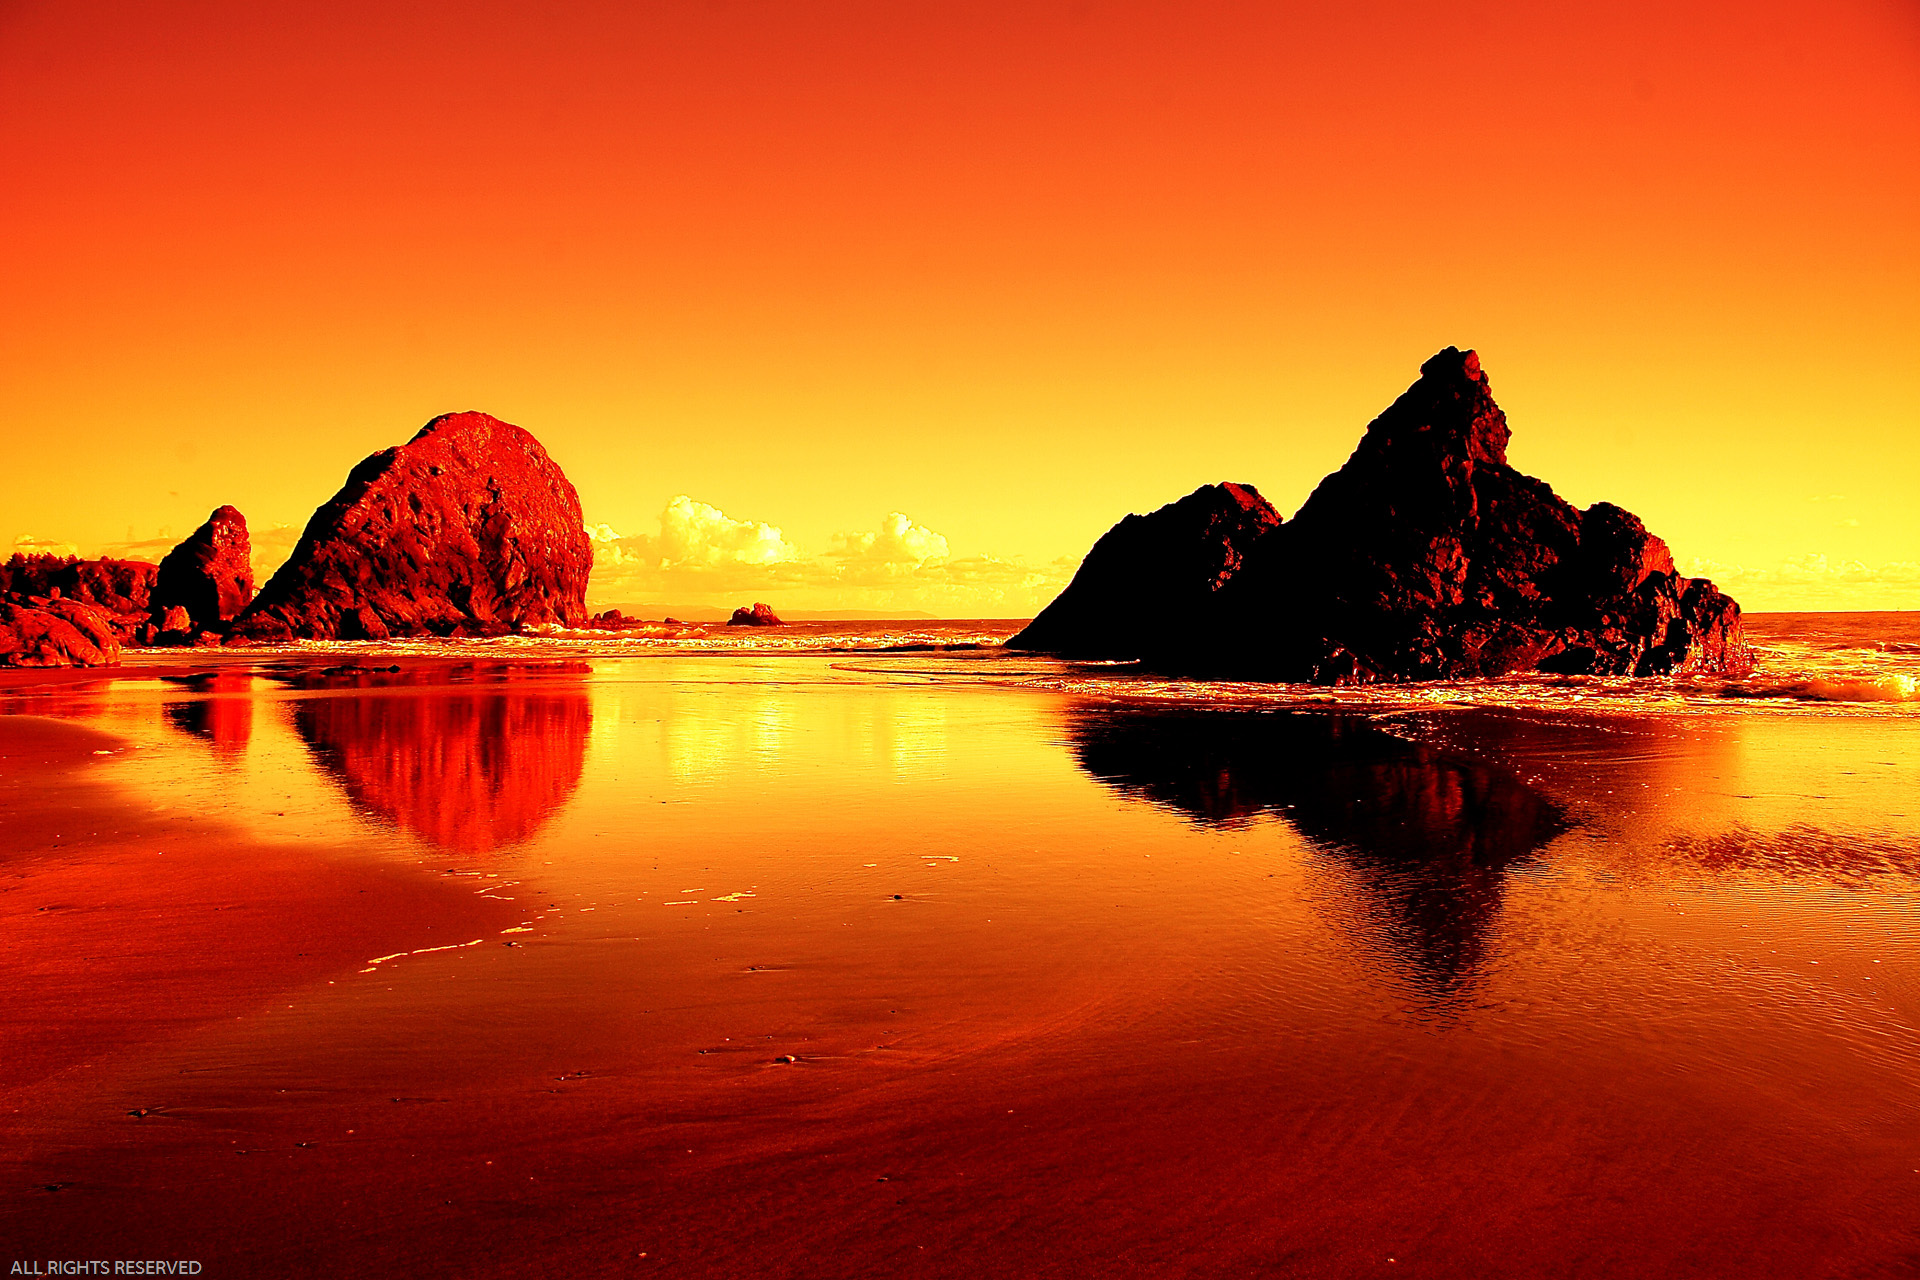
\includegraphics[width=\linewidth]{images/sunset.jpg}
		\caption{Beautiful Sea Sunset}
	\end{SCfigure}
	
	
	
	\chapter{Content}
	\lipsum[2]
	\lipsum[3]
	
	\section{First Section}
	\subsection{Subsection}
	
	\lipsum[2]
	
	\lipsum[2]
	
	\lipsum[3]
	
	\sideTable[A flat table example]{
		\begin{tabu} to \marginparwidth {XX}
			\tableHeaderStyle
			Key & Value\\
			key 1 & value 1\\
			key 2 & value 2\\
			key 3 & value 3\\
			key 4 & value 4\\
		\end{tabu}
	}
	\subsection{Second Section}
	
	\lipsum[2-3]
	
	\sideQuote[Julius Caesar]{\lipsum[2]}
	\lipsum[3-4]
	
	
	
	\begin{descr}
		\itemColor{Rome}\lipsum[3]
		\itemColor{Democracy} \lipsum[4]
		\itemColor{Soldier} \lipsum[27]
	\end{descr}
	
	\warningInfo{InfoBulle --- Warning}{\lipsum[3]}
	
	\newpage
	\begin{figure}[ht!]
		\begin{whole}
			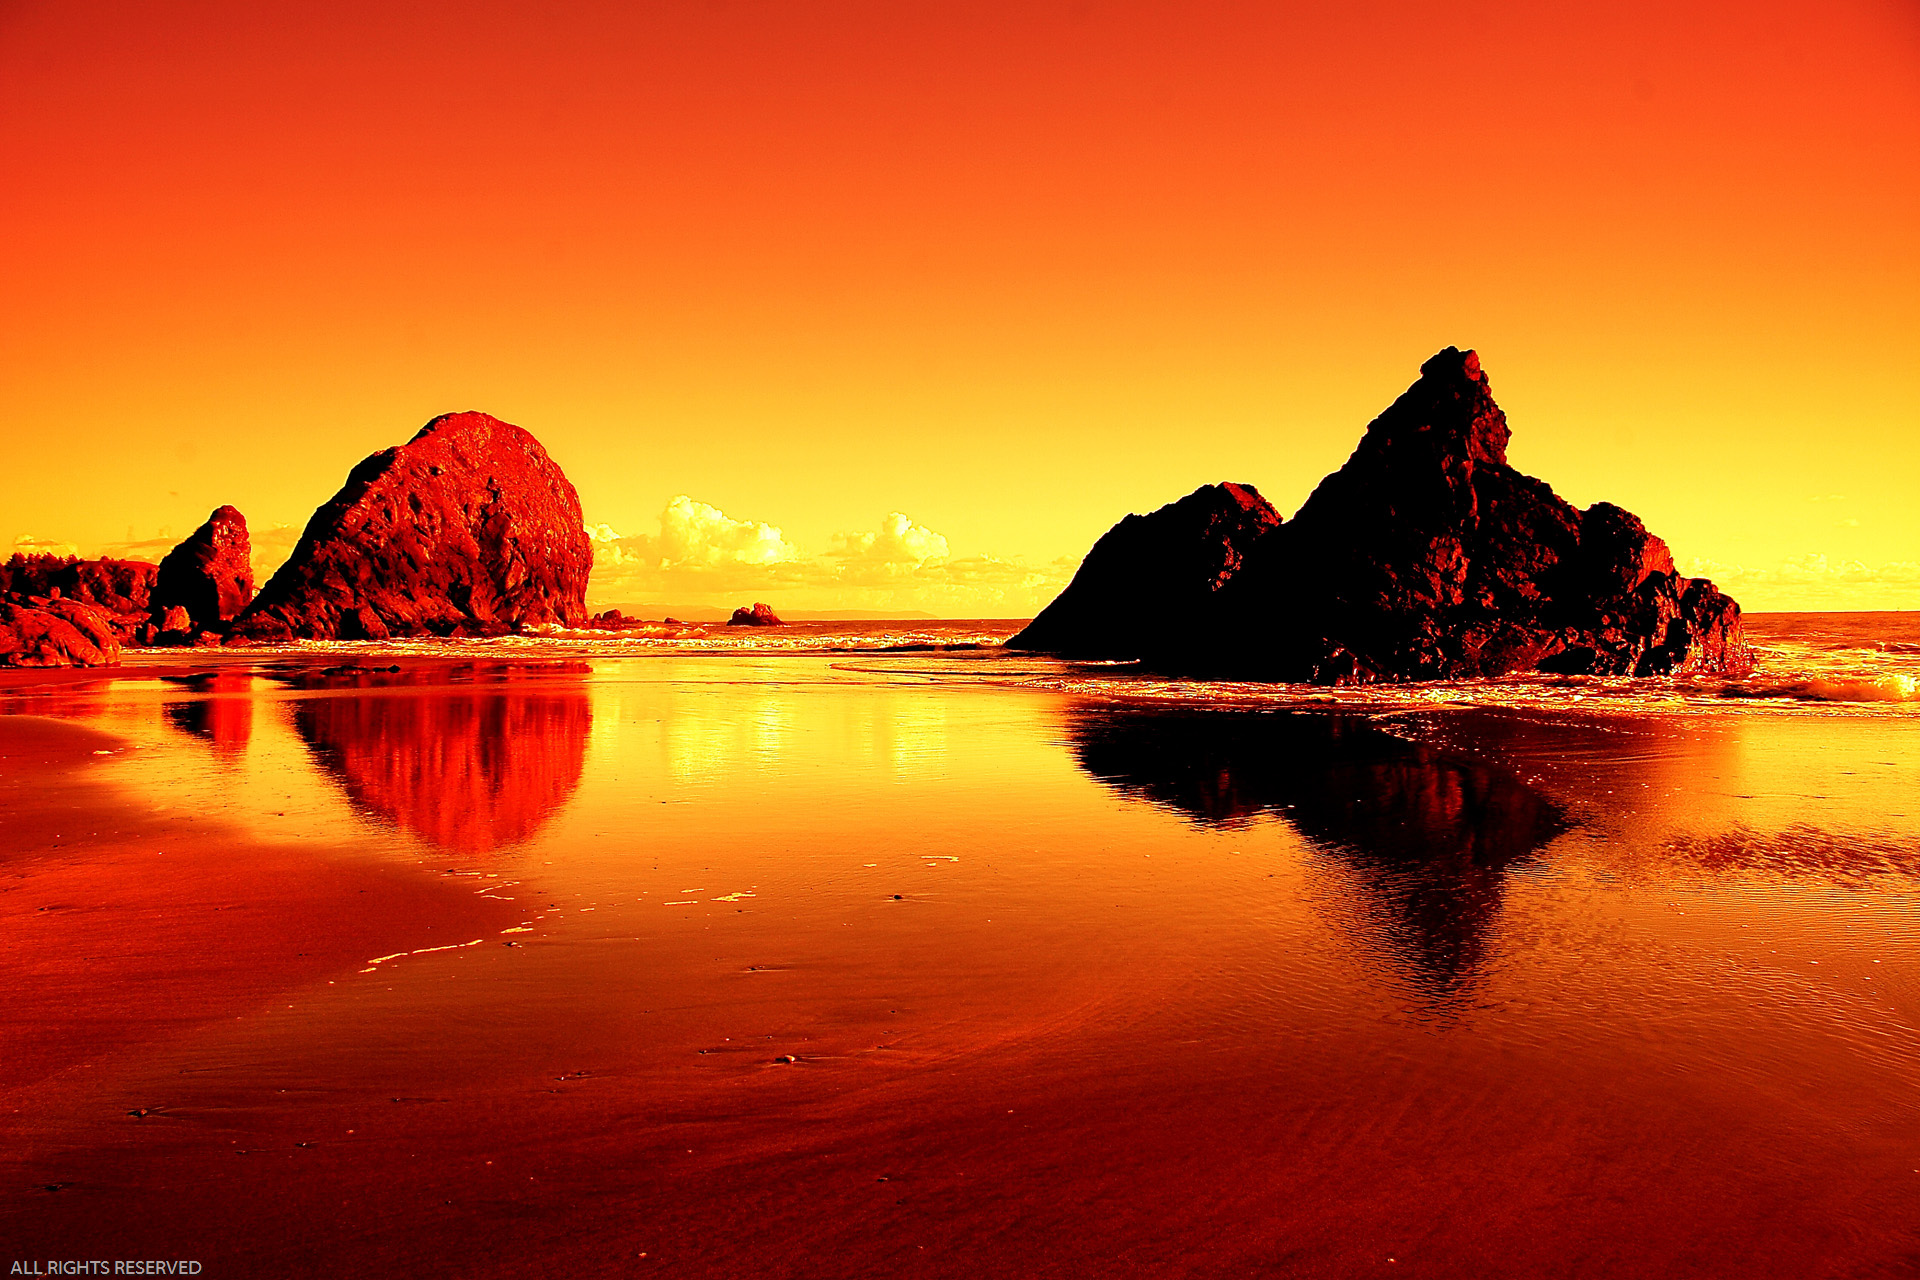
\includegraphics[width=\linewidth]{images/sunset.jpg}
			\caption{Beautiful Sea Sunset}
		\end{whole}
	\end{figure}
	
	\lipsum[10]
	
	\begin{items}
		\item \lipsum[2]
		\item \lipsum[3]
		\sideFigure[Beautiful Sea Sunset]{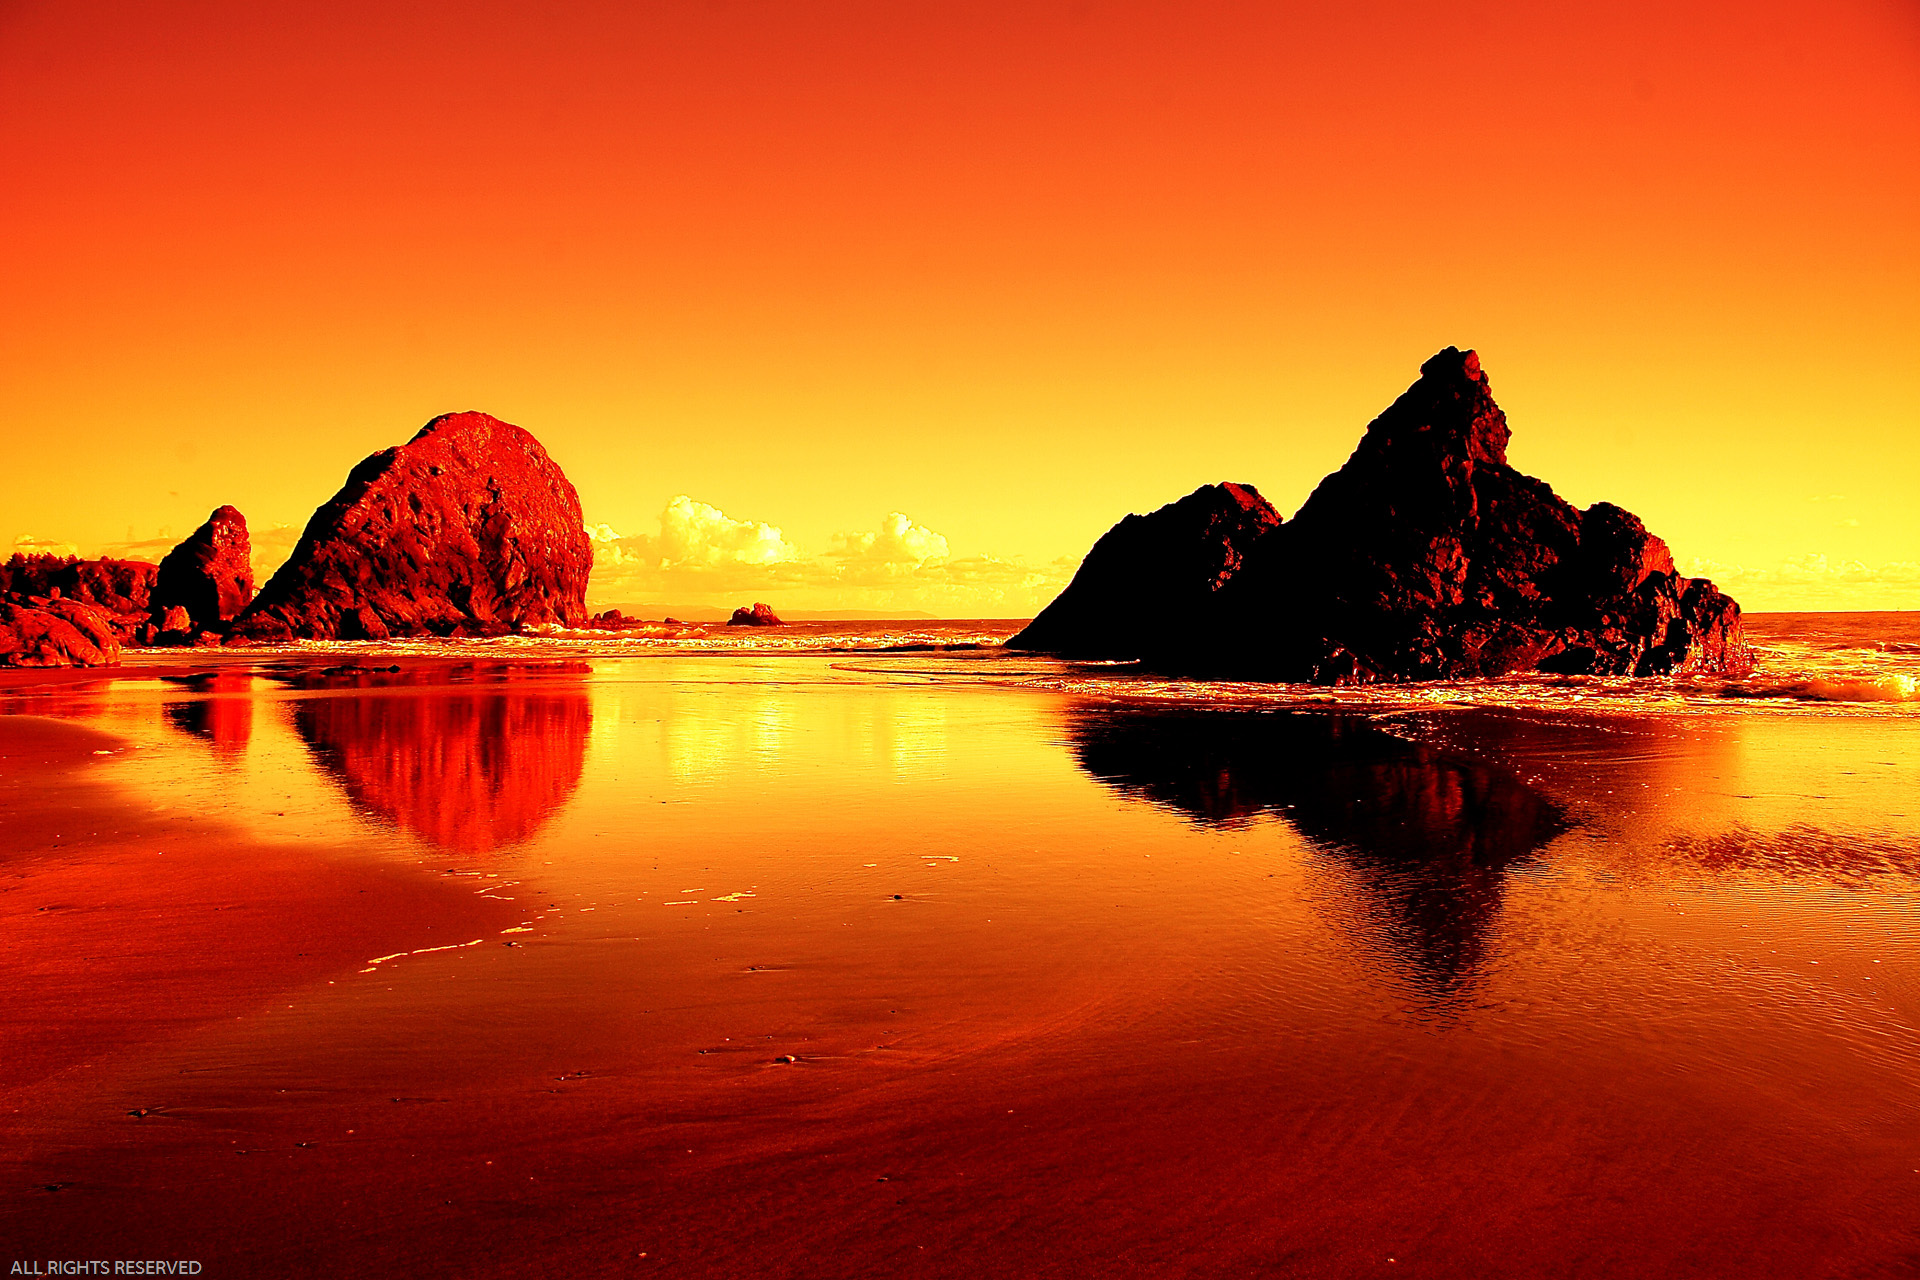
\includegraphics[width=\linewidth]{images/sunset.jpg}}
		\item \lipsum[2]
		\item \lipsum[7]
	\end{items}
	
	\criticalInfo{Title}{\lipsum[3]}
\end{document}